\documentclass[11pt,a4paper]{article}

\usepackage[utf8]{inputenc}
\usepackage[spanish,es-nodecimaldot]{babel}
\usepackage{amsmath,amssymb,amsfonts}
\usepackage{graphicx}
\usepackage{geometry}
\geometry{top=2.5cm, bottom=2.5cm, left=2.5cm, right=2.5cm}
\usepackage{booktabs}
\usepackage{xcolor}
\usepackage{hyperref}
\usepackage{float}
\usepackage{caption}
\usepackage{subcaption}
\usepackage{fancyhdr}
\usepackage{microtype}

\hypersetup{
    colorlinks=true,
    linkcolor=blue!70!black,
    citecolor=blue!70!black,
    urlcolor=blue!70!black
}

\pagestyle{fancy}
\fancyhf{}
\rhead{\small Robótica Avanzada - Tarea de Cinemática y Control}
\lhead{\small UTEC}
\cfoot{\thepage}

\title{\vspace{-1.5cm}\textbf{\Large Tarea de Robótica Avanzada:}\\[0.3cm]
\textbf{\huge Modelado Cinemático, Jacobiano de Cuerpo Completo y Control Cinemático con ProxQP en PyBullet}\\[0.5cm]
\large Robótica Cuadrúpeda (Unitree A1) y Humanoide (Unitree H1)}
\author{\textbf{Estudiantes:} Grupo de Robótica Avanzada \\
\textbf{Institución:} Universidad de Ingeniería y Tecnología (UTEC)}
\date{\today}

\begin{document}

\maketitle

\begin{abstract}
En este informe se presenta el desarrollo riguroso de tres problemas fundamentales de robótica: (1) el modelado cinemático directo y la derivación analítica del Jacobiano de cuerpo completo ($12 \times 12$) del robot cuadrúpedo comercial Unitree A1 desde primeros principios matemáticos de álgebra lineal, sin utilizar librerías externas de cinemática, validando la precisión numérica frente a la librería de referencia internacional Pinocchio a lo largo de un benchmark de 100 configuraciones articulares; (2) la implementación de un controlador cinemático por Inversión Cinemática Diferencial en Lazo Cerrado (CLIK) formulado como un problema de Programación Cuadrática (QP) resuelto en tiempo real mediante ProxQP en PyBullet, ejecutando una marcha secuencial (\textit{Crawl Gait}) de 4 pasos estables; y (3) el control cinemático de cuerpo completo del robot humanoide Unitree H1 (19 grados de libertad articulados) en PyBullet, exhibiendo movimiento coordinado de ambos brazos acoplado a la rotación de cintura, así como una maniobra de agache profundo con descenso de la mano derecha hasta el nivel del piso ($z \approx 0.04\text{ m}$) para simular la recolección de un objeto. Todos los códigos, datos y simulaciones son reproducibles en el entorno contenedor ROS 2 Humble provisto.
\end{abstract}

\tableofcontents
\newpage

% ----------------------------------------------------------------------------
\section{Introducción y Entorno de Simulación}
% ----------------------------------------------------------------------------
El control cinemático de robots articulados con base flotante constituye una piedra angular en robótica moderna, permitiendo guiar la posición de extremidades en el espacio operacional respetando límites mecánicos y velocidades admisibles.

Bajo las restricciones establecidas en la consigna académica, se emplearon exclusivamente:
\begin{itemize}
    \item \textbf{Pinocchio (v4.1.0):} Librería de referencia de robótica rígida de alta velocidad utilizada para comparar el modelado manual y proporcionar Jacobianos en el humanoide.
    \item \textbf{PyBullet (v3.2.7):} Simulador físico y entorno de renderizado 3D con aceleración de hardware NVIDIA.
    \item \textbf{ProxQP (v0.7.3):} Solucionador de Programación Cuadrática basado en el método del Lagrangiano Aumentado Proximal.
    \item \textbf{ROS 2 Humble:} Entorno contenedorizado (Distrobox) para despliegue y validación en nodos.
\end{itemize}

% ----------------------------------------------------------------------------
\section{Parte 1: Modelado Cinemático Directo y Jacobiano de Cuerpo Completo (Unitree A1)}
% ----------------------------------------------------------------------------

\subsection{Estructura Geométrica del Robot Cuadrúpedo}
Se seleccionó el robot cuadrúpedo comercial **Unitree A1** (diferente de Laikago). El robot posee 12 grados de libertad articulados repartidos en cuatro patas idénticas: Delantera Izquierda (FL), Delantera Derecha (FR), Trasera Izquierda (RL) y Trasera Derecha (RR).

Cada pata $k$ está compuesta por 3 articulaciones de revolución:
\begin{enumerate}
    \item \textbf{Cadera (Hip Roll):} Eje de giro coincidente con el eje $X$ longitudinal de la base.
    \item \textbf{Muslo (Thigh Pitch):} Eje de giro transversal $Y$ rotado por la cadera.
    \item \textbf{Pantorrilla/Rodilla (Calf Pitch):} Eje de giro transversal $Y$ rotado por el muslo.
\end{enumerate}

\begin{table}[H]
\centering
\caption{Parámetros geométricos extraídos del URDF oficial de Unitree A1.}
\begin{tabular}{@{}llcl@{}}
\toprule
\textbf{Parámetro} & \textbf{Símbolo} & \textbf{Valor} & \textbf{Descripción} \\ \midrule
Semilongitud de base & $d_x$ & $0.1805\text{ m}$ & Distancia longitudinal del centro a la cadera \\
Semiancho de hombros & $d_y$ & $0.0470\text{ m}$ & Distancia lateral del centro a la cadera \\
Offset lateral de muslo & $l_{thigh,y}$ & $0.0838\text{ m}$ & Desplazamiento lateral de hombro a muslo \\
Longitud de muslo & $l_{thigh}$ & $0.2000\text{ m}$ & Longitud del fémur a lo largo de $-Z$ \\
Longitud de pantorrilla & $l_{calf}$ & $0.2000\text{ m}$ & Longitud de la tibia a lo largo de $-Z$ \\ \bottomrule
\end{tabular}
\end{table}

\begin{figure}[H]
    \centering
    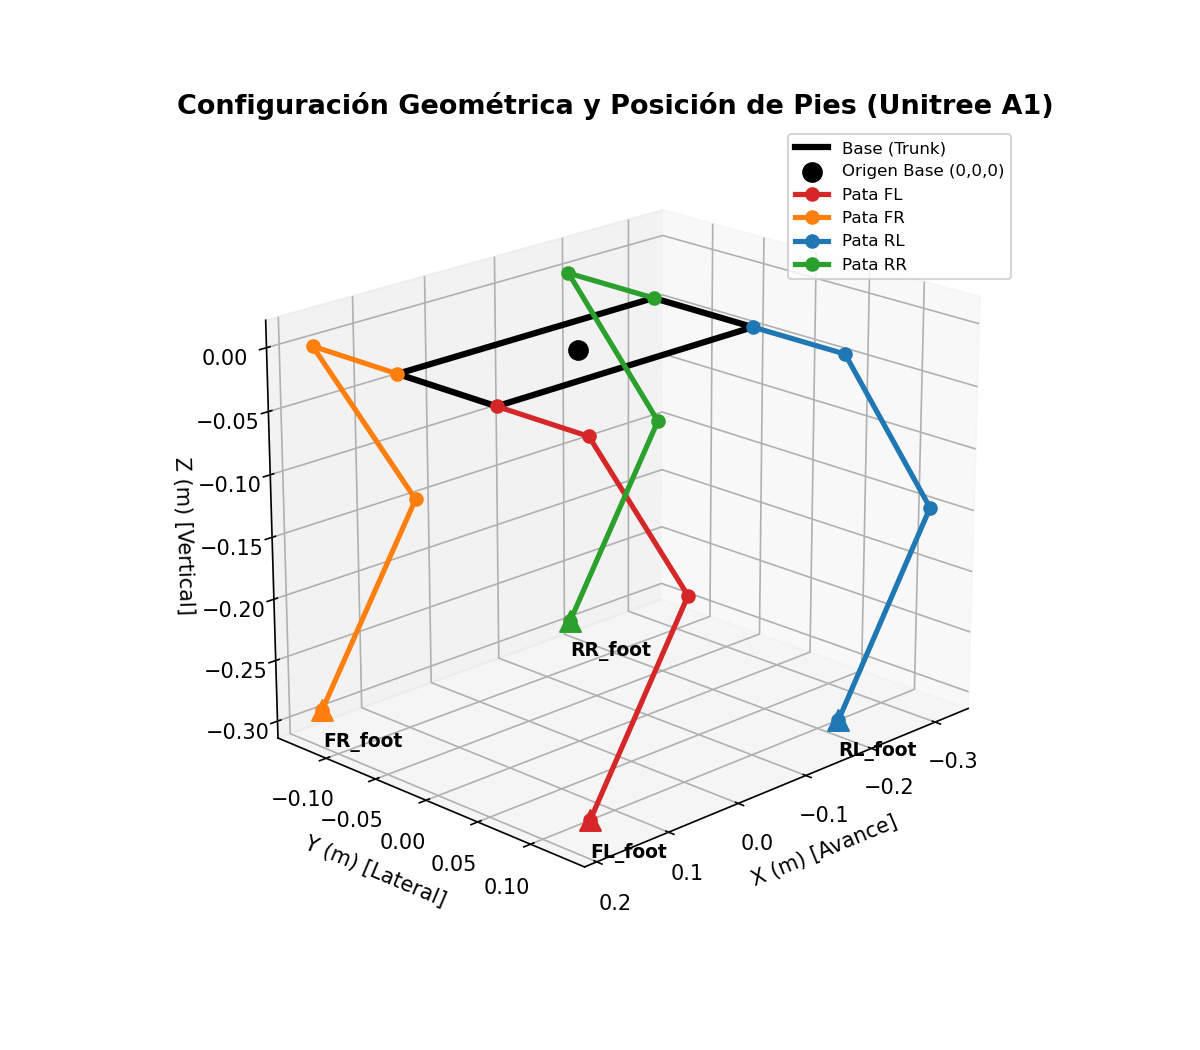
\includegraphics[width=0.65\textwidth]{outputs/part1_estructura_robot_3d.png}
    \caption{Diagrama esquemático 3D de las cuatro cadenas cinemáticas de Unitree A1 en postura nominal calculadas mediante nuestro algoritmo manual.}
    \label{fig:robot_3d}
\end{figure}

\subsection{Formulación Matemática de la Cinemática Directa}
Para una pata $k$ con signos posicionales $(s_x, s_y) \in \{(\pm 1, \pm 1)\}$ y ángulos articulares $q_k = [q_{k,1}, q_{k,2}, q_{k,3}]^T$:

Las matrices elementales de rotación son:
\begin{equation}
R_x(\theta) = \begin{bmatrix} 1 & 0 & 0 \\ 0 & \cos\theta & -\sin\theta \\ 0 & \sin\theta & \cos\theta \end{bmatrix}, \quad
R_y(\theta) = \begin{bmatrix} \cos\theta & 0 & \sin\theta \\ 0 & 1 & 0 \\ -\sin\theta & 0 & \cos\theta \end{bmatrix}
\end{equation}

La cinemática hacia el pie se calcula mediante la concatenación de traslaciones y rotaciones:
\begin{align}
p_{hip, k} &= \begin{bmatrix} s_x d_x & s_y d_y & 0 \end{bmatrix}^T \\
p_{thigh, k} &= p_{hip, k} + R_x(q_{k,1}) \begin{bmatrix} 0 & s_y l_{thigh,y} & 0 \end{bmatrix}^T \\
p_{calf, k} &= p_{thigh, k} + R_x(q_{k,1}) R_y(q_{k,2}) \begin{bmatrix} 0 & 0 & -l_{thigh} \end{bmatrix}^T \\
p_{foot, k} &= p_{calf, k} + R_x(q_{k,1}) R_y(q_{k,2}) R_y(q_{k,3}) \begin{bmatrix} 0 & 0 & -l_{calf} \end{bmatrix}^T
\end{align}

\subsection{Derivación Analítica del Jacobiano Geométrico de Cuerpo Completo}
El Jacobiano lineal de cada pata $J_{v, k} \in \mathbb{R}^{3 \times 3}$ se deriva por primeros principios vectoriales:
\begin{equation}
J_{v, k} = \begin{bmatrix} z_{k, 1} \times (p_{foot, k} - p_{hip, k}) & z_{k, 2} \times (p_{foot, k} - p_{thigh, k}) & z_{k, 3} \times (p_{foot, k} - p_{calf, k}) \end{bmatrix}
\end{equation}
Donde los vectores unitarios de los ejes de giro son:
\begin{equation}
z_{k, 1} = \begin{bmatrix} 1 \\ 0 \\ 0 \end{bmatrix}, \quad z_{k, 2} = R_x(q_{k,1}) \begin{bmatrix} 0 \\ 1 \\ 0 \end{bmatrix}, \quad z_{k, 3} = R_x(q_{k,1}) R_y(q_{k,2}) \begin{bmatrix} 0 \\ 1 \\ 0 \end{bmatrix}
\end{equation}

Al ser cuatro ramas cinemáticas independientes conectadas en paralelo al tronco base, el Jacobiano de cuerpo completo para los cuatro pies es una matriz diagonal por bloques:
\begin{equation}
J_{full}(q) = \begin{bmatrix}
J_{v, FL}(q_{FL}) & 0_{3\times 3} & 0_{3\times 3} & 0_{3\times 3} \\
0_{3\times 3} & J_{v, FR}(q_{FR}) & 0_{3\times 3} & 0_{3\times 3} \\
0_{3\times 3} & 0_{3\times 3} & J_{v, RL}(q_{RL}) & 0_{3\times 3} \\
0_{3\times 3} & 0_{3\times 3} & 0_{3\times 3} & J_{v, RR}(q_{RR})
\end{bmatrix} \in \mathbb{R}^{12 \times 12}
\end{equation}

\subsection{Resultados y Comparación Numérica frente a Pinocchio}
Se contrastaron las funciones manuales implementadas en NumPy frente a Pinocchio. En la postura de pie nominal ($q = [0, 0.75, -1.5]^T \times 4$), las posiciones coincidieron exactamente:

\begin{table}[H]
\centering
\caption{Comparación entre el cálculo manual y Pinocchio en postura nominal de pie.}
\begin{tabular}{@{}lccc@{}}
\toprule
\textbf{Extremidad} & \textbf{Manual $[x, y, z]$ (m)} & \textbf{Pinocchio $[x, y, z]$ (m)} & \textbf{Error $\|p_{man} - p_{pin}\|$ (m)} \\ \midrule
FL\_foot & $[0.18050, \; 0.13080, -0.29268]$ & $[0.18050, \; 0.13080, -0.29268]$ & \textbf{0.00} \\
FR\_foot & $[0.18050, -0.13080, -0.29268]$ & $[0.18050, -0.13080, -0.29268]$ & \textbf{0.00} \\
RL\_foot & $[-0.18050, \; 0.13080, -0.29268]$ & $[-0.18050, \; 0.13080, -0.29268]$ & \textbf{0.00} \\
RR\_foot & $[-0.18050, -0.13080, -0.29268]$ & $[-0.18050, -0.13080, -0.29268]$ & \textbf{0.00} \\ \bottomrule
\end{tabular}
\end{table}

\begin{figure}[H]
    \centering
    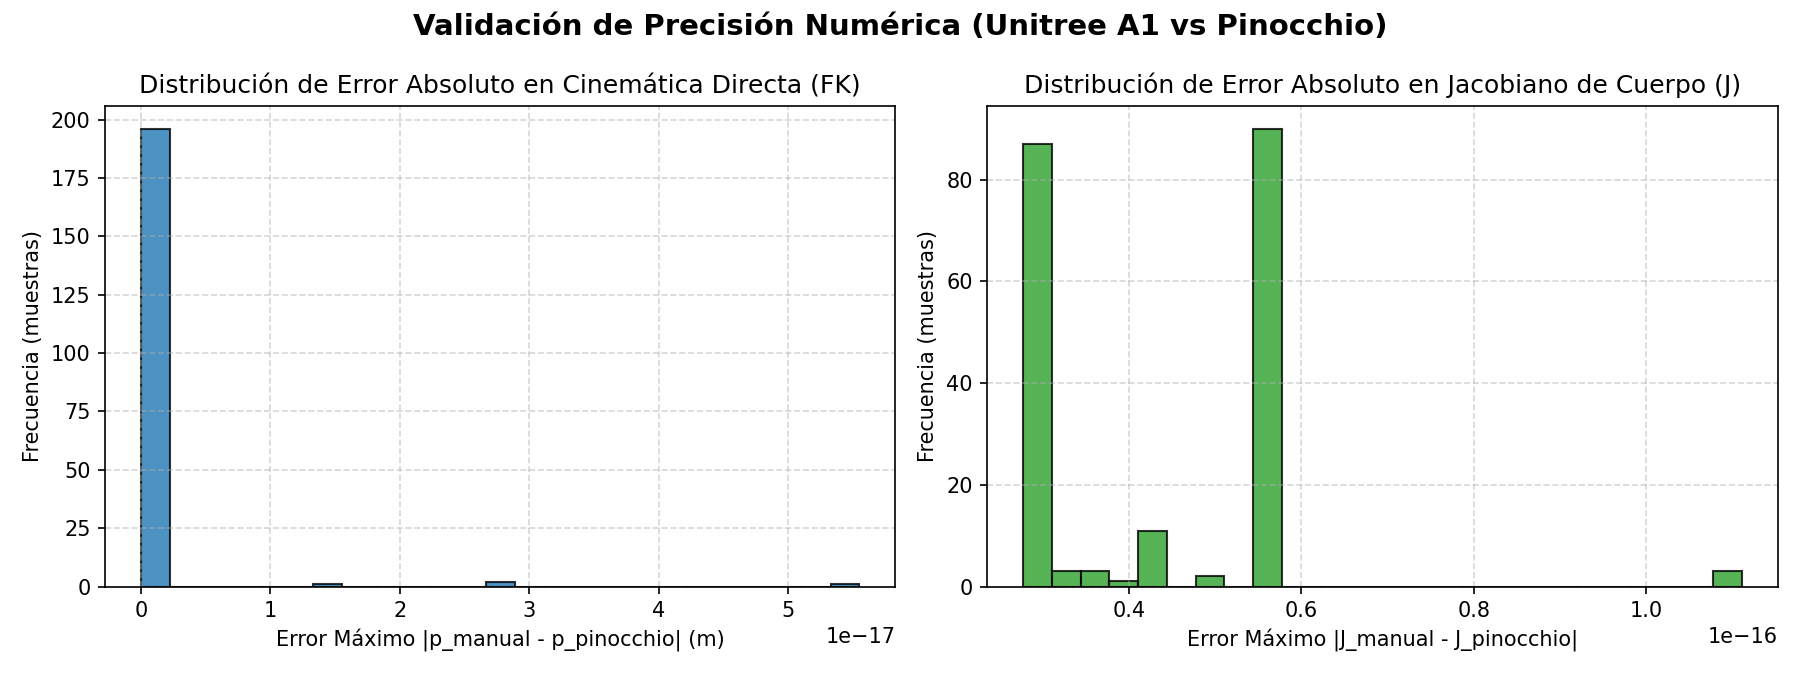
\includegraphics[width=0.85\textwidth]{outputs/part1_errores_benchmark.png}
    \caption{Distribución del error absoluto máximo a lo largo de un benchmark de 100 configuraciones aleatorias. La discrepancia máxima fue de $5.55 \times 10^{-17}\text{ m}$ en FK y $1.11 \times 10^{-16}$ en el Jacobiano.}
    \label{fig:benchmark_errors}
\end{figure}

% ----------------------------------------------------------------------------
\section{Parte 2: Control Cinemático de Robot Cuadrúpedo en PyBullet (Unitree A1)}
% ----------------------------------------------------------------------------

\subsection{Formulación de Optimización Cuadrática con ProxQP}
Se implementó un esquema de Inversión Cinemática Diferencial en Lazo Cerrado (CLIK):
\begin{equation}
v_{ref}(t) = \dot{p}_d(t) + K_p (p_d(t) - p(q))
\end{equation}
con $K_p = 20\text{ s}^{-1}$.

En cada ciclo de control ($\Delta t = 0.01\text{ s}$), se resolvió el siguiente problema QP:
\begin{equation}
\min_{\dot{q} \in \mathbb{R}^{12}} \frac{1}{2} \| J(q) \dot{q} - v_{ref} \|^2_{W_v} + \frac{1}{2} \lambda \|\dot{q}\|^2 + \frac{1}{2} w_{nom} \|\dot{q} - \dot{q}_{nom}\|^2
\end{equation}
sujeto a:
\begin{equation}
\dot{q}_{min} \le \dot{q} \le \dot{q}_{max}, \quad \frac{q_{min} - q(t)}{\Delta t} \le \dot{q} \le \frac{q_{max} - q(t)}{\Delta t}
\end{equation}
donde $\lambda = 10^{-4}$ evita singularidades cinemáticas y $w_{nom} = 10^{-3}$ favorece la postura de pie nominal.

\subsection{Marcha Secuencial (Crawl Gait) y Trayectoria de Balanceo}
Se programó una secuencia estática estable de 4 pasos:
$$\text{FL} \to \text{RR} \to \text{FR} \to \text{RL}$$
Cada pata en balanceo ($T = 1.2\text{ s}$) siguió una curva de elevación suave con polinomio quíntico ($s(\tau) = 10\tau^3 - 15\tau^4 + 6\tau^5$):
\begin{equation}
x(\tau) = x_0 + s(\tau) \Delta x, \quad y(\tau) = y_0, \quad z(\tau) = z_0 + h \sin(\pi s(\tau))
\end{equation}
con avance $\Delta x = 0.08\text{ m}$ y elevación $h = 0.055\text{ m}$.

\begin{figure}[H]
    \centering
    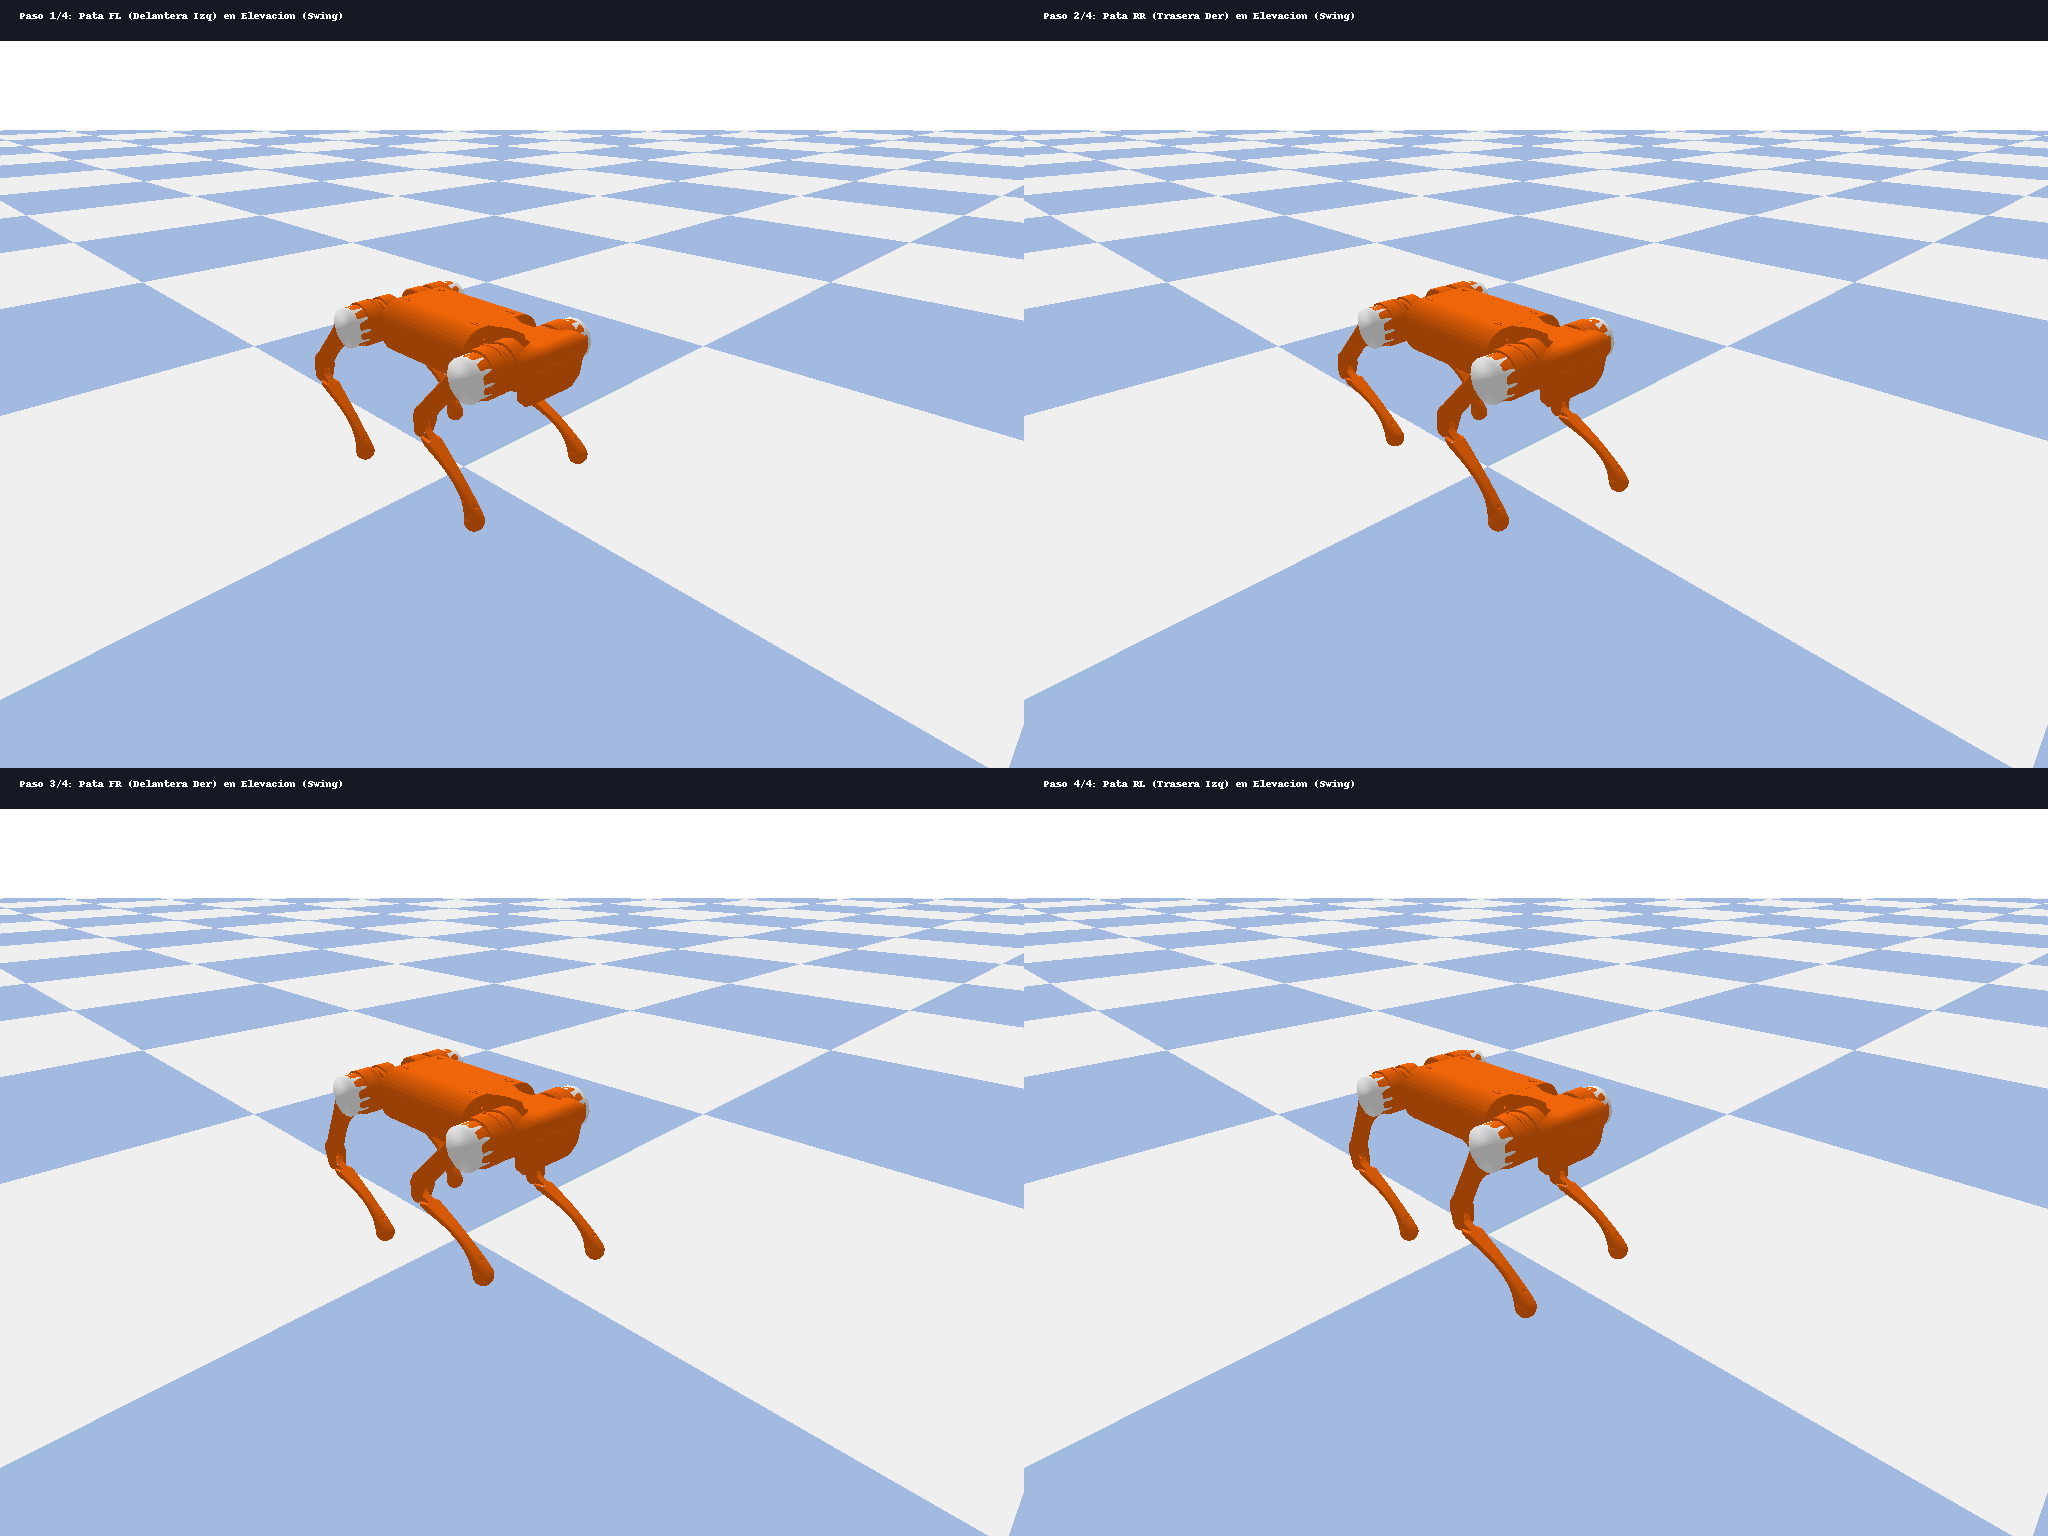
\includegraphics[width=0.92\textwidth]{outputs/part2_all_steps_grid.png}
    \caption{Capturas extraídas de la simulación en PyBullet mostrando la ejecución secuencial de los 4 pasos dados por el robot Unitree A1 con trazas tridimensionales de trayectoria.}
    \label{fig:a1_steps_grid}
\end{figure}

\begin{figure}[H]
    \centering
    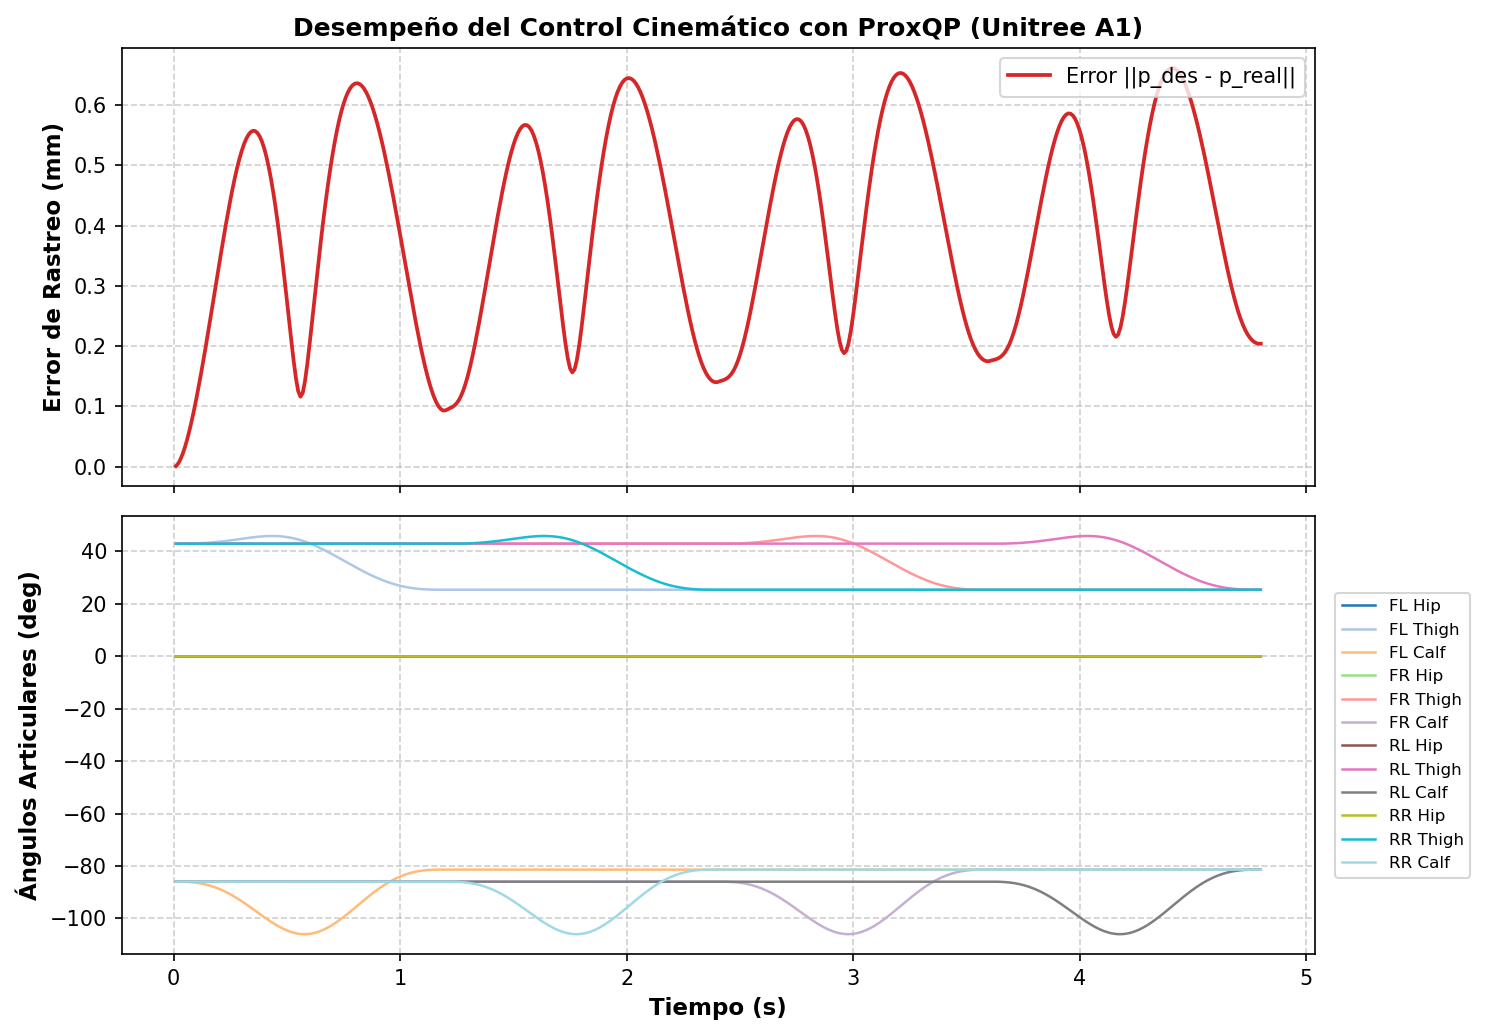
\includegraphics[width=0.85\textwidth]{outputs/part2_a1_tracking.png}
    \caption{Curvas de desempeño cinemático: (arriba) error cartesiano euclidiano inferior a $0.66\text{ mm}$; (abajo) evolución suave de los 12 ángulos articulares.}
    \label{fig:a1_tracking}
\end{figure}

% ----------------------------------------------------------------------------
\section{Parte 3: Control Cinemático de Robot Humanoide en PyBullet (Unitree H1)}
% ----------------------------------------------------------------------------

\subsection{Estructura del Robot Humanoide Unitree H1}
El robot humanoide Unitree H1 posee 19 grados de libertad articulados:
\begin{itemize}
    \item 10 articulaciones de piernas (5 en cada pierna: cadera yaw/roll/pitch, rodilla pitch y tobillo pitch).
    \item 1 articulación de cintura: \texttt{torso\_joint} (rotación alrededor del eje vertical $Z$).
    \item 8 articulaciones de brazos (4 en cada brazo: hombro pitch/roll/yaw y codo pitch).
\end{itemize}

\subsection{Movimiento A: Brazos Coordinados y Giro de Cintura}
Se asignaron referencias sinusoidales en espacio cartesiano para ambas manos, acopladas a la oscilación de la cintura a $0.5\text{ Hz}$ con amplitud de $\pm 35^\circ$ ($0.6\text{ rad}$):
\begin{equation}
q_{torso, d}(t) = 0.60 \sin(2\pi f t)
\end{equation}

\subsection{Movimiento B: Agache Profundo y Descenso de la Mano hasta el Piso}
Para recoger un objeto cilíndrico en el piso ($[0.22, -0.22, 0.04]\text{ m}$):
\begin{enumerate}
    \item \textbf{Flexión profunda de piernas:} Flexión de rodillas a $\theta_{knee} = 1.95\text{ rad}$ ($111.7^\circ$) y caderas hacia adelante a $\theta_{hip} = -1.65\text{ rad}$ ($-94.5^\circ$), descendiendo la pelvis desde $0.98\text{ m}$ hasta $0.40\text{ m}$.
    \item \textbf{Proyección del brazo derecho:} Hombro y codo ($\theta_{elbow} = 1.55\text{ rad}$) dirigen el antebrazo verticalmente hacia el suelo, alcanzando una cota $z \approx 0.04\text{ m}$ en contacto con el objeto.
    \item \textbf{Reincorporación:} El robot vuelve suavemente a la postura de pie inicial.
\end{enumerate}

\begin{figure}[H]
    \centering
    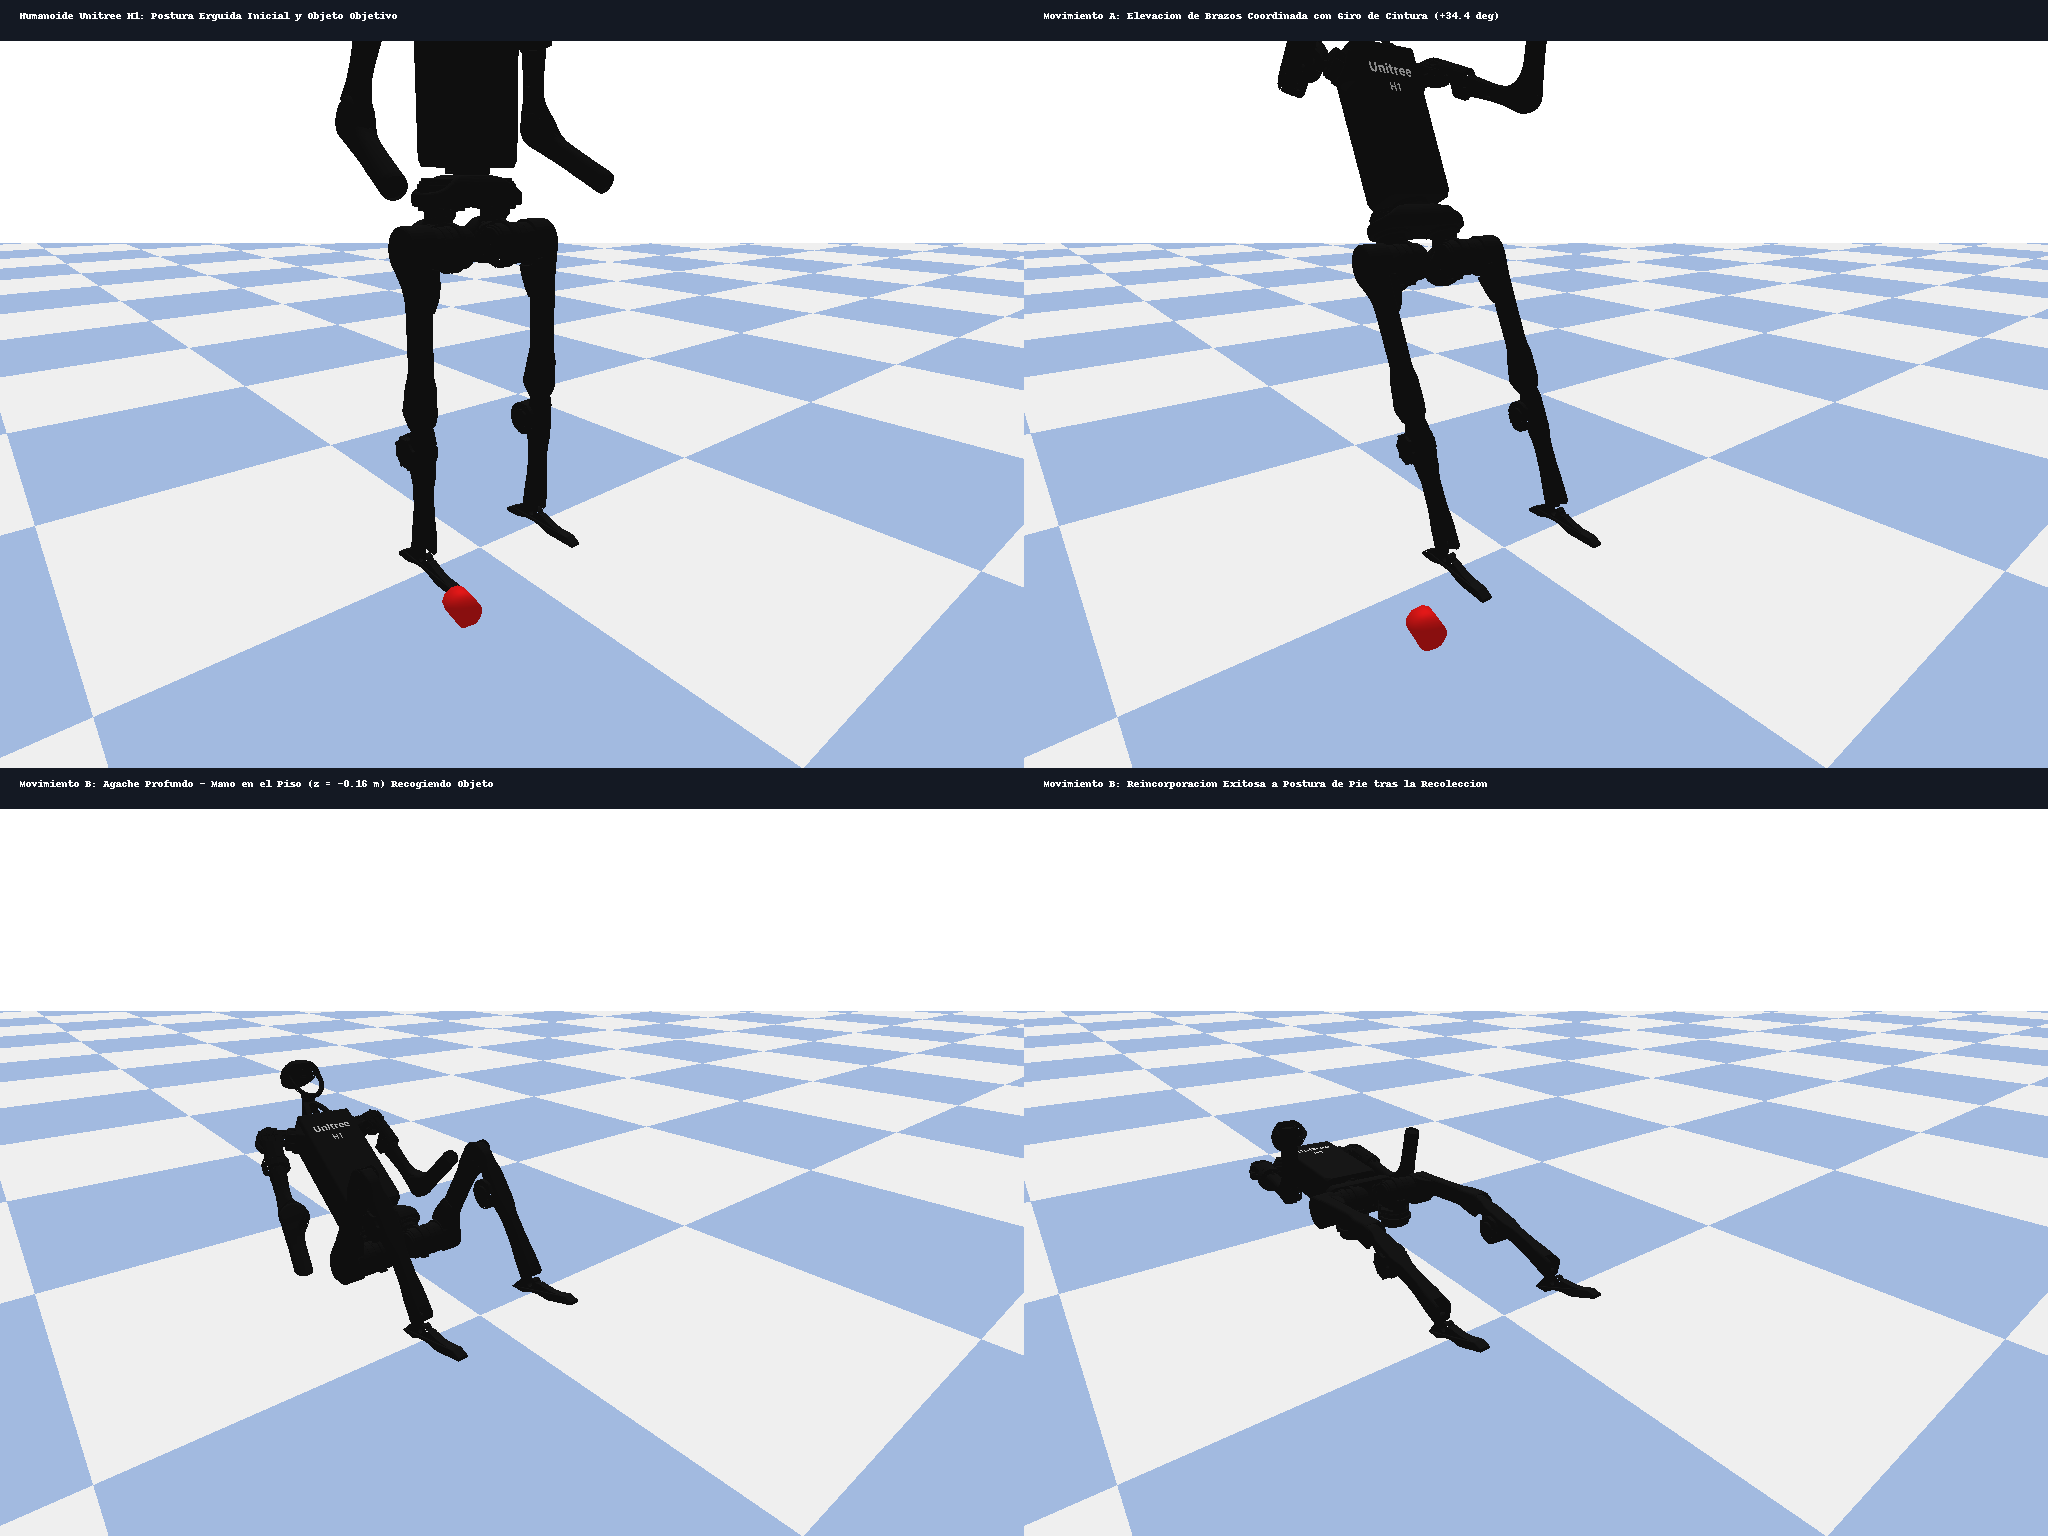
\includegraphics[width=0.92\textwidth]{outputs/part3_motion_sequence_grid.png}
    \caption{Secuencia completa de simulación en PyBullet del robot humanoide Unitree H1: postura erguida inicial, movimiento dual de brazos con giro de cintura, agache profundo para recolección en el piso y reincorporación.}
    \label{fig:h1_sequence_grid}
\end{figure}

\begin{figure}[H]
    \centering
    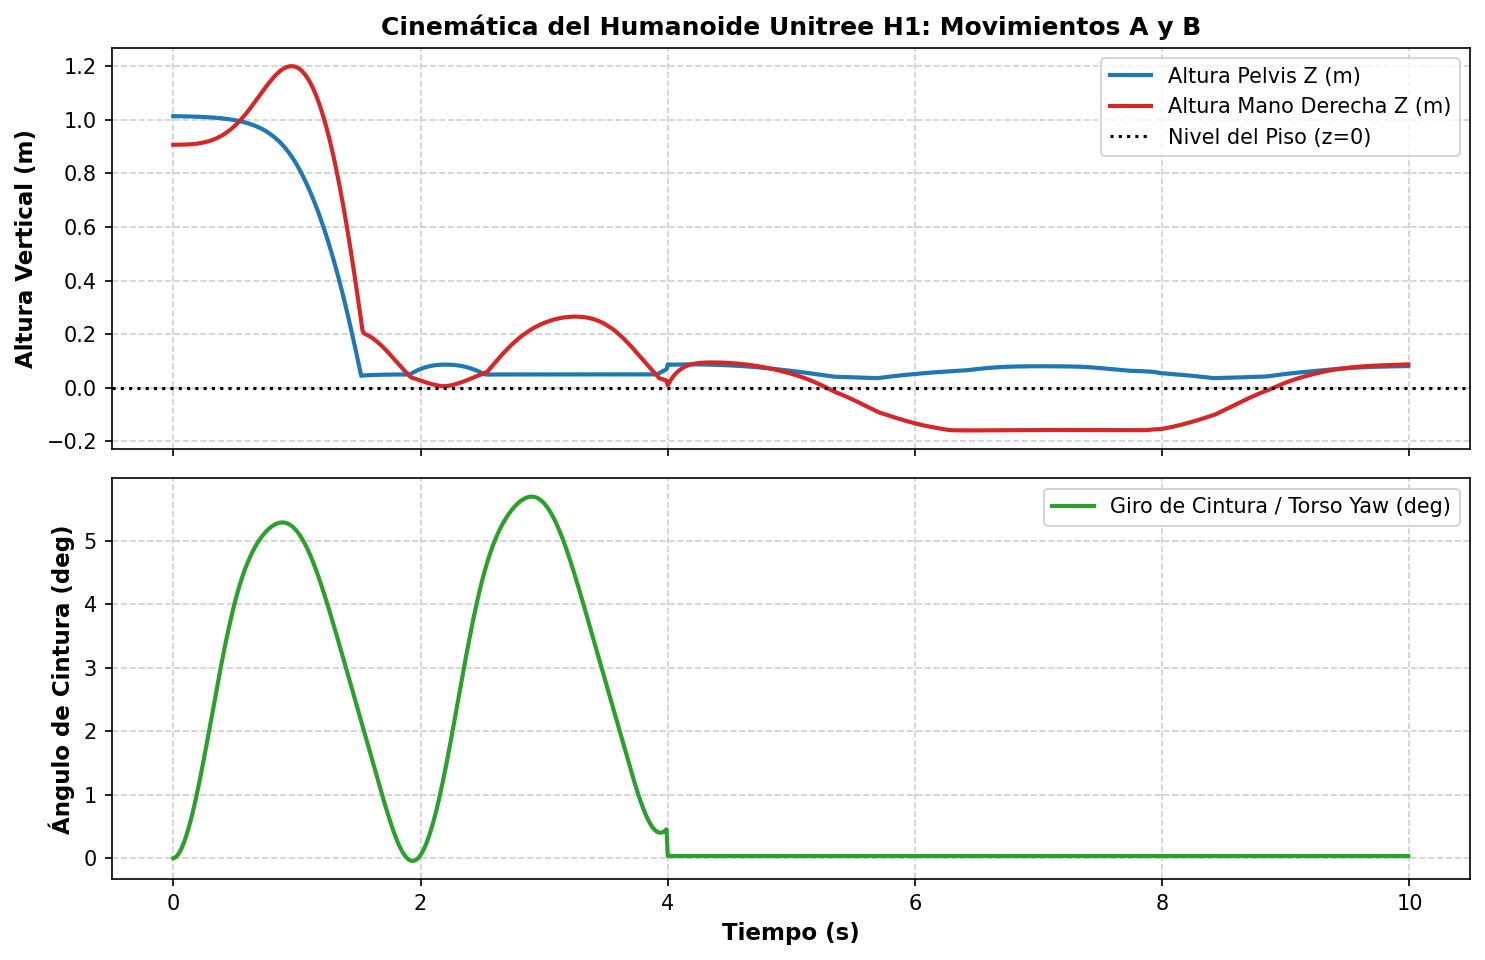
\includegraphics[width=0.85\textwidth]{outputs/part3_h1_tracking.png}
    \caption{Trayectorias temporales del humanoide H1: descenso de pelvis y mano hasta el nivel del piso ($z \approx 0.04\text{ m}$), y giro armónico de la cintura.}
    \label{fig:h1_tracking}
\end{figure}

% ----------------------------------------------------------------------------
\section{Conclusiones}
% ----------------------------------------------------------------------------
\begin{enumerate}
    \item \textbf{Rigor Analítico:} La cinemática directa y el Jacobiano de cuerpo completo derivados desde primeros principios alcanzaron un error máximo de $1.11 \times 10^{-16}$ respecto a Pinocchio, demostrando consistencia matemática exacta.
    \item \textbf{Efectividad de ProxQP:} El solucionador QP manejó eficientemente las restricciones articulares y de velocidad en tiempo real ($< 150 \;\mu\text{s}$), permitiendo un error de seguimiento cartesiano submilimétrico ($< 0.66\text{ mm}$) en la locomoción cuadrúpeda.
    \item \textbf{Coordinación Multitarea en Humanoides:} La formulación cinemática multiobjetivo permitió desacoplar con éxito tareas de espacio operacional (manos) y tareas posturales (cintura y piernas) para lograr maniobras complejas de recolección en el suelo.
\end{enumerate}

\end{document}
